% !TEX encoding = UTF-8 Unicode
%%%%%%%%%%%%%%%%%%%%%%%%%%%%%%%%%%%%%%%%%
% Beamer Presentation
% LaTeX Template
% Version 1.0 (10/11/12)
%
% This template has been downloaded from:
% http://www.LaTeXTemplates.com
%
% License:
% CC BY-NC-SA 3.0 (http://creativecommons.org/licenses/by-nc-sa/3.0/)
%
%%%%%%%%%%%%%%%%%%%%%%%%%%%%%%%%%%%%%%%%%

%----------------------------------------------------------------------------------------
%	PACKAGES AND THEMES
%----------------------------------------------------------------------------------------

\documentclass[9pt, xelatex]{beamer}

\mode<presentation> {

% The Beamer class comes with a number of default slide themes
% which change the colors and layouts of slides. Below this is a list
% of all the themes, uncomment each in turn to see what they look like.


%\usetheme{default}
%\usetheme{AnnArbor}
%\usetheme{Antibes}
%\usetheme{Bergen}
%\usetheme{Berkeley}
%\usetheme{Berlin}
\usetheme{Boadilla}
%\usetheme{CambridgeUS}
%\usetheme{Copenhagen}
%\usetheme{Darmstadt}
%\usetheme{Dresden}
%\usetheme{Frankfurt}
%\usetheme{Goettingen}
%\usetheme{Hannover}
%\usetheme{Ilmenau}
%\usetheme{JuanLesPins}
%\usetheme{Luebeck}
%%\usetheme{Madrid}
%\usetheme{Malmoe}
%\usetheme{Marburg}
%\usetheme{Montpellier}
%\usetheme{PaloAlto}
%\usetheme{Pittsburgh}
%\usetheme{Rochester}
%\usetheme{Singapore}
%\usetheme{Szeged}
%\usetheme{Warsaw}

% As well as themes, the Beamer class has a number of color themes
% for any slide theme. Uncomment each of these in turn to see how it
% changes the colors of your current slide theme.

%\usecolortheme{albatross}
%\usecolortheme{beaver}
%\usecolortheme{beetle}
%\usecolortheme{crane}
%\usecolortheme{dolphin}
%\usecolortheme{dove}
%\usecolortheme{fly}
%\usecolortheme{lily}
%\usecolortheme{orchid}
%\usecolortheme{rose}
%\usecolortheme{seagull}
%\usecolortheme{seahorse}
%\usecolortheme{whale}
%\usecolortheme{wolverine}
\bibliographystyle{plain} %abbrvnat
\usepackage{natbib}
\usepackage{epstopdf}
\usepackage{graphicx} % Allows including images
\usepackage{booktabs} % Allows the use of \toprule, \midrule and \bottomrule in tables
\usepackage{amsmath} 
\usepackage{amssymb}
\usepackage{multirow}
\usepackage{amsthm}
%\usepackage {tikz}
\usepackage {xcolor}
\usepackage {kotex}
\usepackage{bm} % To use bold math symbol
\definecolor {processblue}{cmyk}{0.96,0,0,0}

%\setbeamertemplate{footline} % To remove the footer line in all slides uncomment this line
\setbeamertemplate{footline}[page number] % To replace the footer line in all slides with a simple slide count uncomment this line
\setbeamertemplate{caption}[numbered]
\setbeamertemplate{itemize item}[ball] % To remove the navigation symbols from the bottom of all slides uncomment this line
}


%----------------------------------------------------------------------------------------
%	TITLE PAGE
%----------------------------------------------------------------------------------------

\title[Short title]{반복측정자료분석 \\
	{\small -일반화선형혼합모형- }
	} % The short title appears at the bottom of every slide, the full title is only on the title page

\author{2020021218 이소연 \\2020020316 황서진} 
% Your name
\institute[]{\small 고려대학교 통계학과} % Your institution as it will appear on the bottom of every slide, may be shorthand to save space

\date{2020.04.13} % Date, can be changed to a custom date

\begin{document}

\begin{frame}
\titlepage % Print the title page as the first slide
\end{frame}

\begin{frame}{Contents}
\frametitle{Contents}
\tableofcontents 
\end{frame}

%----------------------------------------------------------------------------------------
%	PRESENTATION SLIDES
%----------------------------------------------------------------------------------------

\section{Introduction}{
	\begin{frame}[allowframebreaks]{Introduction}
		\textcolor{black}{\textbf{경시적 자료에 대한 전통적인 ANOVA 방법의 한계}}
		\vspace{5mm}
		
		\begin{itemize}
			\item 모든 개체들이 같은 시점과 같은 반복 횟수를 가정한다.
			\item 시간 가변 공변량(time-varying covariate)의 적용에 한계를 가진다.
			\item 결측자료의 효과를 반영하는 방법이 많지 않다.
			\vspace{5mm}
			
			$\Longrightarrow$ 보다 일반화된 반복측정 자료 분석 모형이 필요하다.
		\end{itemize}
		
		\framebreak
		\textcolor{black}{\textbf{선형모형의 확장}}
		\vspace{5mm}
		
		종속변수가 정규분포를 따르지 않는다면?
		\vspace{2mm}
		
		$\Longrightarrow$ \textbf{Generalized Linear Model}(GLM)
		\vspace{5mm}
		
		관측치 간 상관관계가 있다면?
		\vspace{2mm}
		
		$\Longrightarrow$ \textbf{Linear Mixed Model}(LMM)
		\vspace{5mm}
		
		관측치가 정규성을 만족하지도 않고, 상관관계까지 있다면?
		\vspace{2mm}
		
		$\Longrightarrow$ \textbf{Generalized Linear Mixed Model}(GLMM)	
		\framebreak
		
		
		\textcolor{black}{\textbf{Defining GLMM}}
		\vspace{2mm}
		\begin{itemize}
			\item Linear Mixed Model: LMM
			\vspace{3mm}
			
			선형 혼합효과모형(LMM)은	$ y_{1},...,y_{n} $ 에 대하여 다음과 같이 표현된다.
			
			\begin{center} $ y_{i}=X_{i}\beta+Z_{i}U_{i}+\epsilon_{i} $\end{center}
			
			X와 Z는 각 고정 효과, 랜덤 효과와 관련된 공변량을 나타내며, $\beta$는 고정 효과, $U$는 랜덤 효과를 나타낸다. $\epsilon$은 오차항을 의미한다.
			\vspace{3mm}
			
			이들은 다음과 같은 가정을 만족한다.
			
			\begin{center}
				$E(U_{i})=0,Var(U_{i})=G$,
				
				$E(\epsilon_{i})=0,		Var(\epsilon_{i})=R_{i},		Cov(U_{i},\epsilon_{i})=0$
			\end{center}
			\vspace{2mm}
			
			$\Rightarrow$ 선형모형 하에서 경시적 자료의 모형화를 위해선 적절한  G와 R에 대한 적용과 \textbf{오차항의 공분산구조의 설정}이 중요하다. 
			\vspace{2mm}
			
			e.g., 균일상관모형, AR(1), ...
		\end{itemize}
		\framebreak
		
		
		\textcolor{black}{\textbf{Defining GLMM}}
		\vspace{2mm}
		\begin{itemize}
			\item Generalized Linear Mixed Model: GLMM
			\vspace{3mm}
			
			선형혼합모형을 이항, 순서형, 이산형 경시적 자료로 확장한다.
			\begin{center}
				\begin{itemize}
					\item \textbf{GLM}과의 차이: 랜덤효과를 추가, 오차항의 공분산구조를 통해 반복치들 간의 연관관계 모형화
					\item \textbf{GEE}와의 차이: 우도함수의 적용 여부와 추정된 회귀계수의 해석
				\end{itemize}
			\end{center}
			
		\end{itemize}
		\framebreak
		
		
		\textcolor{black}{\textbf{Defining GLMM}}
		\vspace{2mm}
		\begin{itemize}
			\item Generalized Linear Mixed Model: GLMM
			\vspace{3mm}
			
			$n$명의 독립적인 관측개체의 반응변수가 $ Y=(y_{1},...,y_{n}) $라고 할 때, 관측개체별 공유되는 특성을 개체별 랜덤 효과 $U_{i}$로 표현한다. 이때, $U_{i}$가 주어져 있다면, 각 개체 내 관측치 $y_{i}=(y_{i1},...,y_{im_{i}})$는 서로 \textcolor{black}{\textbf{독립}} 이라고 가정한다. 
			
			즉, \textbf{조건부 독립(conditional independence)}를 가정한다.
			\vspace{2mm}
			
			각 관측치의 평균을 $ E(y_{ij}|U_{i})=\mu_{ij}$ 라고 할 때, \textbf{연결함수}(link function) g에 의해 다음과 같이 표현될 수 있다.
			
			\begin{center} $g(\mu_{ij})=X_{ij}\beta+Z_{ij}U_{i}$\end{center}
			\vspace{2mm}
			
			여기서 $X_{ij}, Z_{ij}$는 각 고정 효과 및 랜덤 효과와 관련된 공변량을 의미하며, 일반적으로 랜덤 효과 $U_{i}$는 평균벡터가 0이고 공분산행렬 $G(\theta)$를 가정한다. 가장 일반적인 선택은 정규분포이다. 
			\vspace{2mm}		
			
		\end{itemize}	
		\framebreak
		
		
		\textcolor{black}{\textbf{Defining GLMM}}
		\vspace{2mm}
		\begin{itemize}
			\item Generalized Linear Mixed Model: GLMM
			\vspace{3mm}
			
			자료의 타입에 따라 다음과 같은 예시를 들 수 있다.
			
			\begin{itemize}
				\item \textbf{이항 경시적 자료}(binary): $Y_{ij}|U_{i} \sim B(1,\mu_{ij}), logit\mu_{ij}=X_{ij}'\beta+Z_{ij}U_{i}$
				\item \textbf{이산형 경시적 자료}(count) $Y_{ij}|U_{i} \sim Poisson(1,\mu_{ij}), log\mu_{ij}=X_{ij}'\beta+Z_{ij}U_{i}$
				\item 가우시안 선형혼합모델 또한 GLMM의 특별한 사례로 간주할 수 있다.
				\begin{center} $Y_{ij}|U_{i} \sim Normal(\mu_{ij},\tau^{2}), \mu_{ij}=X_{ij}'\beta+Z_{ij}U_{i}$
				\end{center}
			\end{itemize}
			\vspace{2mm}
			
			공분산구조는 그룹 간 변동(among-group variation)과 그룹 내 자기 상관 잔차(autocorrelated residuals)로 구분될 수 있다.
			\vspace{2mm}
			
			GLMM은 보다 다양한 경시적 자료 분석 모형에 랜덤효과를 추가하여, 오차항의 공분산구조 $\Sigma$ (e.g., $\Sigma_{AR(1)}$)를 통해 반복치들 간의 연관관계 모형화할 수 있다.
			
		\end{itemize}	
	\end{frame}
}


\section{The Salamander Mating Experiments}{
	\begin{frame}[allowframebreaks]{The Salamander Mating Experiments}
		\begin{center}
			\graphicspath{ {./} }
			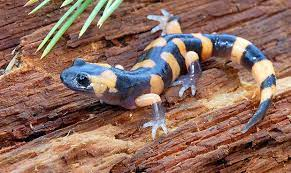
\includegraphics[scale=0.6]{sal}
			\vspace{4mm}
			
			두 타입의 도롱뇽 모집단: Rough Butt (R) and White Side (W)
			\vspace{3mm}
			
			$\surd$ Do salamanders prefer mating with their own population?
		\end{center}
		
		
		\framebreak
		
		
		\textbf{실험계획} \\
		\vspace{4mm}
		\begin{itemize}
			\item 각 도롱뇽은 두 타입의 파트너와 모두 매칭됨 (반복 측정)
			\vspace{2mm}
			\item 각 도롱뇽은 짝짓기에 대한 개별적인 성향을 가지고 있으며, 이는 측정할 수 없음
			\vspace{2mm}
			\item 각 도롱뇽의 성향은 독립적이라고 가정
			\vspace{4mm}
			
			\item 도롱뇽이 짝짓기를 할 확률에 영향을 미치는 효과:
			\begin{itemize}
				\item 페어링 타입 (RR, RW, WR, WW) (고정 효과)
				\item 암컷의 개별 짝짓기 성향 (랜덤 효과)
				\item 수컷의 개별 짝짓기 성향 (랜덤 효과)
			\end{itemize}
		\end{itemize}
		
		\framebreak
		\textbf{실험계획} \\
		\vspace{4mm}
		\begin{itemize}
			
			\item 반응변수: 짝짓기 유무 (Binary)
			\item 고정효과: $\beta_{RR}, \beta_{RW}, \beta_{WR}, \beta_{WW}$ (짝짓기 확률의 로그 오즈)
			\item 랜덤효과: 개별 성향 반영, 서로 독립이고 정규분포를 따른다고 가정
			\item 추정 분산: $\sigma_{F}^{2}, \sigma_{M}^{2}$
			
		\end{itemize}
		\vspace{5mm}
		
		$\triangleright$ How?
		
		
	\end{frame}
}


\section{Estimation of Parameters}{
	\begin{frame}[allowframebreaks]{Estimation of Parameters}
		\textbf{Likelihood based Inference}
		\vspace{4mm}
		
		\begin{itemize}
			\item $y_{i}=(y_{i1},...,y_{im_{i}}, U_{i})$의 결합 분포(Joint):
			
			\begin{center}
				$f(y_{i},U_{i};\beta,\theta)=f(U_{i};\theta)f(y_{i}|U_{i},\beta)=f(U_{i};\theta)\prod_{j=1}^{m_{i}} f(y_{ij}|U_{i},\beta)$
			\end{center}
			\vspace{2mm}
			
			\item $y_{i}$의 주변분포(Marginal):
			
			\begin{center}
				$f(y_{i},U_{i};\beta,\theta)=\int f(U_{i};\theta)\prod_{j=1}^{m_{i}} f(y_{ij}|U_{i},\beta)dU_{i}$
			\end{center}
			\vspace{2mm}
			
			\item 우도함수(Likelihood):
			
			\begin{center}
				$L(\beta,\theta; y)=\prod_{i=1}^{n}\int f(U_{i};\theta)\prod_{j=1}^{m_{i}} f(y_{ij}|U_{i},\beta)dU_{i}$	
			\end{center}
			
			\vspace{2mm}
			
			$y_{ij}$가 정규분포라면 위 적분의 계산이 비교적 간단한 반면, 대부분의 경우 closed form이 존재하지 않고 복잡하다.
			\vspace{2mm}
			
			이 경우 크게 (1) \textbf{구적법}(Quadrature), (2) \textbf{우도함수의 근사화}, (3) \textbf{몬테카를로}(Monte Carlo) 방법을 사용한다.
		\end{itemize}
		
		\framebreak
		\textbf{수치적 방법: 구적법}
		\vspace{4mm}
		
		구적에 의한 근사화는 피적분함수의 가중치합(weighted sum)이다. 이때 여러가지 구적법 중 \textbf{Gauss-Hermite}(GHQ)와 \textbf{adaptive Gaussian}(AGQ) 구적법이 가장 많이 쓰인다.
		\vspace{2mm}
		
		\begin{center}
			$\int^{\infty}_{-\infty} e^{-x^{2}}f(x)dx \approx \sum^{R}_{k=1}w_{k}f(a_{k})$
		\end{center}
		
		\begin{itemize}
			\item 다항함수로 근사화될 수 있는 $f$에 대한 적분은 $R$개의 가중치합으로 근사화될 수 있으며, 여기서 $a_{k}$는 \textbf{구적점}(quadrature point), $w_{i}$는 \textbf{구적 가중치}(quadrature weight)라고 한다.
			\item GHQ 방법에서는 구적점이 고정된 반면, AGQ 방법에서는 구적접의 위치를 피적분 함수의 형태에 따라 변화시킴으로써 적분의 정확성을 향상시키고자 한다.
			\item SAS의 GLIMMIX 모형의 경우, GHQ 방법 또는 1차 테일러 시리즈 근사를 통해 적분을 근사시킨다.
		\end{itemize}
		\framebreak
		\textbf{수치적 방법: 구적법}
		\vspace{4mm}
		
		예를 들어, 다음의 모형을 가정하였을 때,
		\begin{center}
			$g(\mu_{ij})=x_{ij}'\beta+U_{i}, U_{i}\sim N(0,\sigma^{2})$
		\end{center}
		\vspace{2mm}
		GHQ 방법에 의해 $L(\beta,\theta; y)$의 적분구간은 다음과 같이 R개의 가중합으로 표현된다.
		\vspace{2mm}
		
		$f(U_{i};\sigma)\to\phi \sim N(0,1)$이 되도록 $U_{i}^{*}=U_{i}/\sigma$로 표준화 한다면,
		\begin{center}
			\begin{align}
				\int f(U_{i};\sigma)\prod_{j=1}^{m_{i}} f(y_{ij}|U_{i})dU_{i} & = \int \phi(U_{i}^{*})\prod_{j=1}^{m_{i}} f(y_{ij}|\sigma,U_{i}^{*})dU_{i}^{*} \\
				& = \int_{-\infty}^{\infty} \frac{1}{\sqrt{2\pi}}e^{-U_{i}^{*2}/2}\prod_{j=1}^{m_{i}} f(y_{ij}|\sigma,U_{i}^{*})dU_{i}^{*}\\
				& \approx \sum_{k=1}^{R}w_{k}^{*}\prod_{j=1}^{m_{i}} f(y_{ij}|\sigma,a_{k}^{*})
			\end{align}
			여기서 $w_{k}^{*}=w_{k}/\sqrt{2\pi}, a_{k}^{*}=\sqrt{2}a_{k}$이다.
		\end{center}
		
		
		\framebreak
		\textbf{우도함수의 근사화}
		\vspace{4mm}
		
		적분을 포함한 우도함수에 대해 \textbf{Laplace} 근사화를 적용할 수 있다.
		\vspace{2mm}
		
		\begin{center}
			Taylor expansion: $q(x)=q(\tilde{x})+\frac{1}{2}q''(\tilde{x})(x-\tilde{x})^{2}$
			
			\begin{align}
				\int^{\infty}_{-\infty} exp(f(x))dx & \approx \int^{\infty}_{-\infty} exp[{f(\tilde{x})-(x-\tilde{x})^{2}}/{2\sigma^{2}}]dx \\
				& =\int^{\infty}_{-\infty}exp(f({\tilde{x}}))\sqrt{2\pi}\sigma\phi(x;\tilde{x},\sigma^{2})dx \\ 
				& =exp(f(\tilde{x}))\sqrt{2\pi}\sigma \\
				& = c|f''(x)|^{-1/2}exp(f(\tilde{x}))
			\end{align}	
		\end{center}
		
		\begin{itemize}
			\item (4)-(6)은 $\phi(x;\tilde{x},\sigma^{2})$는 평균이 $\tilde{x}$이고 분산이 $\sigma^{2}$인 정규분포일때, $\tilde{x}$가 f(x)의 최빈값으로 $f'(\tilde{x})=0$이고 $f''(\tilde{x})=1/\sigma^{2}$임을 적용했다.
			
		\end{itemize}
		\framebreak
		\textbf{우도함수의 근사화}
		\vspace{4mm}
		
		\textbf{Laplace} 근사화를 GLMM의 적분에 적용한다.
		\vspace{2mm}
		
		\begin{center}
			$L(\beta,\theta; y)=\prod_{i=1}^{n}\int f(U_{i};\theta)\prod_{j=1}^{m_{i}} f(y_{ij}|U_{i},\beta)dU_{i}$
			\vspace{3mm}
			
			$\Rightarrow$
			$f(U_{i};\theta)\prod_{j=1}^{m_{i}} f(y_{ij}|U_{i}) = exp\{log[(U_{i};\theta)\prod_{j=1}^{m_{i}} f(y_{ij}|U_{i})]\}$
		\end{center}
		\vspace{4mm}
		
		\begin{itemize}
			
			\item 라플라스 근사화에서 정의된 최빈값($\tilde{x}$)은 다음과 같다.
			\vspace{1mm}
			
			\begin{center}
				$\tilde{U_{i}}=argmax{f((U_{i};\theta)\prod_{j=1}^{m_{i}} f(y_{ij}|U_{i})}$
			\end{center}
			\vspace{1mm}
			
		\end{itemize}
		\framebreak
		\textbf{우도함수의 근사화}
		\vspace{4mm}
		
		\begin{itemize}
			\item (1)-(3)의 정규분포 예시에 Laplace 근사화를 적용해보면, 다음과 같다.
			\begin{center}
				\begin{align}
					logf(y_{i};\beta,\sigma) & \approx log(\sqrt{2\pi}\sigma_{i})+log(\phi(\tilde{U_{i}};\sigma))+\sum logf(y_{ij}|\tilde{U_{i}})\\
					& =log(\sigma_{i}/\sqrt{\sigma})-\tilde{U_{i}^{2}}/2\sigma+\sum_{j=1}^{m_{i}}logf(y_{ij}|U_{i})
				\end{align}
			\end{center}
			
			\item MLE를 보장하진 않는다.
			\vspace{2mm}
			
			\item 랜덤 효과가 정규분포를 따를 때만 적용할 수 있다.
			\vspace{2mm}
			
			\item 데이터가 sparse하면 성능이 좋지 않을 수 있다.
		\end{itemize}
		\framebreak
		\textbf{우도함수의 근사화}
		\vspace{4mm}
		
		\textbf{Penalized Quasi-Likelihood}(PQL) 근사화
		\vspace{2mm}
		
		\begin{itemize}
			\item Laplace 근사화의 일반화된 방법이다.
			\vspace{2mm}
			
			\item  $U_{i} \sim N(0,G)$가 주어져 있을 때, 각 개체 내 관측치 $y_{i}=(y_{i1},...,y_{im_{i}})$가 서로 \textcolor{black}{\textbf{조건부 독립}} 이라는 가정 하에 PQL 근사화 식은 다음과 같이 정의된다.
			\vspace{1mm}
			
			\begin{center} $L_{Q} \propto |G|^{-1/2} \int exp \{-\frac{1}{2}\sum_{j=1}^{m_{i}}d_{ij}-\frac{1}{2}U_{i}'G^{-1}U_{i} \}dU_{i}$
			\end{center}
			\vspace{2mm}
			
			여기서 $E(y_{ij}|U_{i})=\mu_{ij}=g^{-1}(X_{ij}\beta+Z_{ij}U_{i})$, 		
			$var(y_{ij}|U_{i})=a_{ij}(\phi)v(\mu_{ij})$일 때 
			
			$\phi$는 산포모수(dispersion parameter), $v(\mu_{ij})$는 알려진 분산 함수라면,
			\vspace{1mm}
			
			\begin{center}
				$d_{ij}=-2\int_{y_{ij}}^{\mu_{ij}}\frac{y_{ij}-u}{a_{ij}(\phi)v(u)}$는 Quasi 분산이다.
			\end{center}
			\vspace{2mm}
			
			\item 위 식의 적분 구간을 Laplace 근사화를 통해 근사한다.
		\end{itemize}
		\framebreak
		\textbf{우도함수의 근사화}
		\vspace{4mm}
		
		\textbf{Penalized Quasi-Likelihood}(PQL) 근사화
		\vspace{2mm}
		
		\begin{itemize}
			\item 우도함수를 근사화하는 방법이기 때문에 MLE를 보장하지 않으며, 추정량이 consistent 하지 않다.
			\vspace{2mm}
			
			\item Laplace 근사법의 한계로 인해 데이터의 분산이 크다면 성능이 좋지 않을 수 있다.
			\vspace{2mm}
			
			\item R의 glmmPQL 패키지를 사용하거나, lme4의 glmer 함수에서 method ="PQL"로 지정하여 사용
			
		\end{itemize}
		\framebreak
	
	\textbf{Monte Carlo Integration} \\
	\vspace{4mm}
	\begin{enumerate}
		\item 단순 몬테칼로 적분법 (Simple Monte Carlo integration) \\
		\vspace{2mm}
		$f_X$로부터 추출된 표본을 이용하여 표본 평균을 구해 기댓값을 근사한다. \\
		\begin{align*}
			& E(h(X)) = \int h(x)f_X(x) dx  \approx \bar{h} = \frac{1}{M}\sum_{\ell=1}^{M}h(\tilde{x_\ell}) \\
			& E(f(y_{ij}\vert \sigma, U_i^*)) = \int \prod_j f(y_{ij}\vert \sigma, U_i^*) dU_i^* 
			\approx	\frac{1}{M}\sum_{\ell=1}^{M}f(y_{ij} \vert \sigma, \tilde{U_{\ell}^*})
		\end{align*}
	
		표본에 의해 발생되는 분산의 증가를 가져오는 단점을 가지게 된다. \\
		\vspace{1mm}
		또한 $f_X$로부터 직접적으로 표본을 추출하는 것이 불가능한 경우 적용불가능하다. 
		
		\framebreak
		
		\item 중요 샘플링 (Importance sampling) \\
		\vspace{2mm}
		단순 몬테칼로 적분법의 단점을 극복하기 위한 대안으로, 적절하게 선택된 중요 함수(importance function) $g$를 이용한다. $g$의 조건은 다음과 같다. \\
		\vspace{1mm}
		\begin{enumerate}
			\item $f_X$와 같은 받침(support)을 가진다. 
			\item $h(x)f_X(x)/g(x)$가 $x$의 smooth 함수이며 제한된 값을 가진다.
			\item $h(x)f_X(x)/g(x)$의 계산이 용이하다. 
		\end{enumerate}
		\vspace{1mm}
		이 때 $h(x)$의 평균은 
		
		\begin{align*}
			& E(h(X)) = \int g(x) \frac{h(x)}{g(x)}f_X(x) dx  \approx \frac{1}{M}\sum_{\ell=1}^{M} \frac{h(\tilde{x_\ell^*})f_X(\tilde{x_{\ell}^*})}{g(\tilde{x_{\ell}^*})} \\
			& E(f(y_{ij}\vert \sigma, U_i^*)) \approx \sum_{\ell=1}^M 
				\frac{\phi(\tilde{U_{\ell}};\mu_i, \tau_i^2)f(y_{ij}\vert \sigma, \tilde{U_\ell})}{\phi(\tilde{U_{\ell}};\mu_i, \tau_i^2)}
		\end{align*}
	\end{enumerate}
	
	\framebreak
		
		\textbf{Monte Carlo EM Algorithm}
		\vspace{2mm}
		\begin{align*}
			& g(\mu_{ij}) = X_{ij}'\beta + Z_{ij}U_i, \quad U_i \sim N(0,\sigma^2)
		\end{align*}
	
		\vspace{4mm} 

		\begin{enumerate}
			\item E-step: \\
				미지의 랜덤 효과와 그 함수를 구하기 위해 조건부 평균 계산.\\
				분포 가정이 없을 경우 Markov chain Monte Carlo (MCMC) 알고리즘 사용. 				
				\begin{align*}
					& Q\{\theta \vert \theta^{(k)} \} = E\{ \log f(y\vert\theta) \vert y, \theta^{(k)}\}
				\end{align*}
			\item M-step: \\
				Newton-Raphson (NR) 기법을 적용해 최대우도추정량 계산.
				\begin{center}
					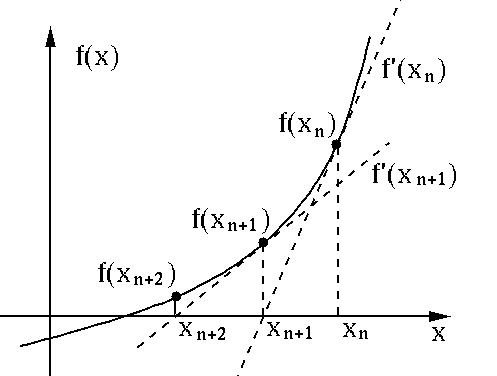
\includegraphics[scale=0.2]{nr.png}
				\end{center}
				% 피셔는 테일러 익스펜션을 활용해 근사해를 구하는데 이때 자코비안을 피셔정보량으로 대체 
		\end{enumerate}
		
	\end{frame}
}

\section{Covariance}{
	\begin{frame}[allowframebreaks]{Modelling the Covariance}
		\textbf{공분산구조}\\
		\vspace{4mm}
		\begin{itemize}
			\item 자료의 종속 구조를 반영하여 연관 관계 파악 가능  
			\item 평균 모형을 구성하는 회귀계수의 표준 오차를 줄임으로써 효율성 향상
		\end{itemize}
	
	\vspace{4mm}
	\textbf{1) 균일상관모형}(Uniform correlation model, compound symemetric, exchangeable) \\
	\vspace{2mm}
	\begin{itemize}
		\item 관측개체 $i$의 모든 반복치 쌍들의 상관관계가 동일
		\begin{align*}
			& Corr(Y_{ij},Y_{ik})=\rho, (i \neq k) \\
			& V_0 = \sigma^2 \vert (1-\rho)I + \rho J \vert 	
%			& Y_{ij} = h(\mu_{ij} + b_i ) + \epsilon_{ij}
		\end{align*} % 구형성 복합대칭
		\item 모든 시간 간격에 대해 동일한 상관계수 가정은 현실적으로 적절하지 않을 수 있음
	\end{itemize}	

	\framebreak
	
	\textbf{2) 지수상관모형}(Exponential correlation model) \\
	\vspace{2mm}	
	\begin{itemize}
		\item 근접한 관측치의 상관관계는 거리가 먼 관측치와의 상관관계보다 강할 것으로 예상됨
		\item 관측 시점이 서로 다른 경우 시간 간격을 고려한 상관계수 고려
		\begin{align*}
			& Cov(Y_{ij},Y_{ik})= \sigma_{jk} = \sigma^2 \exp (-\phi \vert t_j - t_k \vert)\, \quad \phi>0
		\end{align*} 
		\item 시간 간격이 일정한 경우 
		\begin{align*}
			& \sigma_{jk} = \sigma^2 \rho_{jk} \\
			& \rho_{jk} = \exp (-\phi \vert j-k \vert), \quad 0 \leq \rho \leq 1
		\end{align*} 
	\end{itemize}	

	\textbf{3) 무구조 상관모형}(Unstructured correlation model) \\
	\vspace{2mm}	
	\begin{itemize}
		\item 분산 공분산의 형태에 제한 없음
		\item 자료에 가장 충실하나 추정해야 할 모수가 많기에 계산적 부담 존재 
		\begin{align*}
			& V_0 = \begin{pmatrix}
				\sigma_1^2 & \sigma_{12} & \cdots & \sigma_{1m} \\
				\sigma_{12} & \sigma_{2}^2 & \cdots & \sigma_{2m} \\
				\vdots & \vdots & \vdots & \vdots \\
				\sigma_{1m} & \sigma_{2m} & \cdots & \sigma_{m}^2 								
			\end{pmatrix}
		\end{align*} 
	\end{itemize}	
	
	\framebreak
	\begin{center}
		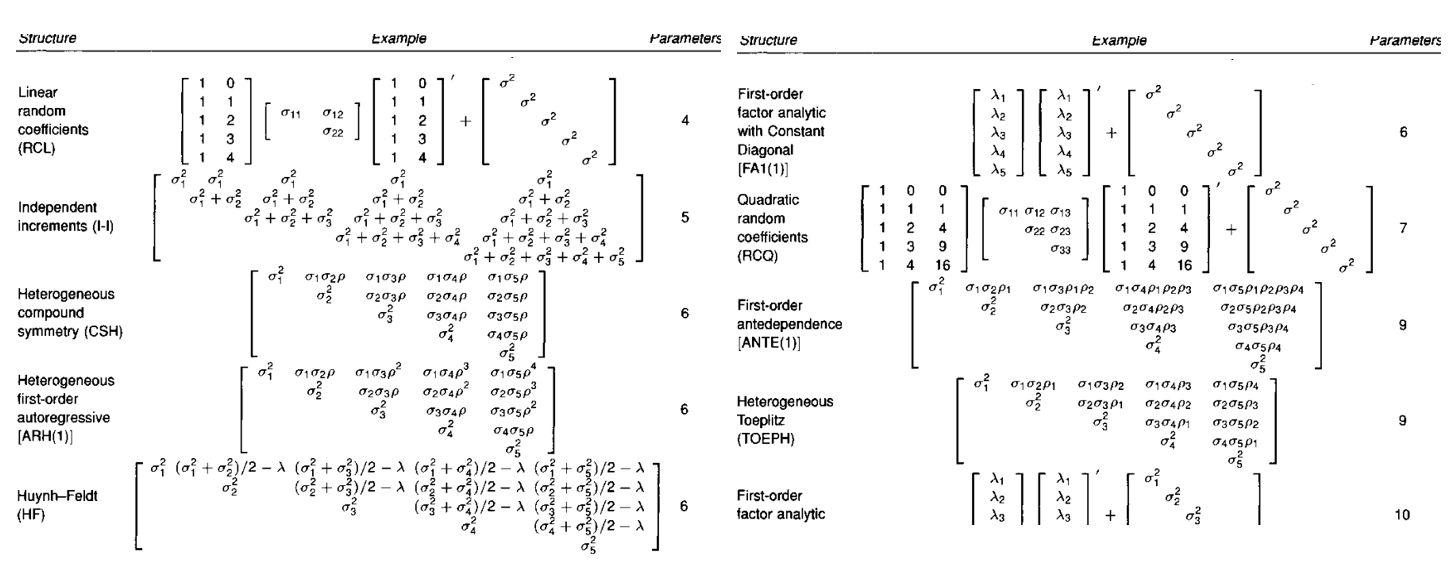
\includegraphics[scale=0.45]{Heterogeneous-Covariance-Structures.png}
	\end{center}
%
%	\framebreak 
%	
%	\textbf{Estimation of Covariance}
%	\begin{align*}
%		V =  \text{Var}(X\beta + & Zb  + \epsilon) =  \text{Var}(Zb+\epsilon) = ZGZ'+R = BLD(V_0) \\
%		&BLD(V_0) = \begin{pmatrix}
%			V_0 & 0 &  \cdots & 0 \\
%			0 & V_0 & \cdots & 0 \\
%			\vdots & \vdots & \ddots 0 \\ 
%			0 & 0 & 0 & V_0
%		\end{pmatrix}
%	\end{align*}
%	\\
%	\vspace{4mm}
%	\begin{itemize}
%		\item Mazimum Likelihood (ML)
%		\item Restricted Maximum Likelihood (REML)
%	\end{itemize}
%
%	\framebreak
%	
%	\textbf{Maximum Likelihood}	
%	\begin{align*}
%		 & \ell(G, R) = \ell(V)  = -\frac{1}{2}\{\log \vert V \vert + (Y-X\beta)'V^{-1}(Y-X\beta) + \frac{n}{2}\log(2\pi) \} \\
%		 & \text{When } V_0 = \sigma^2V_1,	\\
%		 & \ell(\beta, \sigma^{2}, V_1)   = -\frac{1}{2}\{ nm \log \sigma^2 + m\log \log \vert V_1 \vert + \sigma^{-2}(Y-X\beta)'V_{1}^{-1}(Y-X\beta) + \frac{n}{2}\log(2\pi) \} 	
%	\end{align*} \\
%\vspace{4mm}
%	1) 간단한 공분산구조 $V_1$을 가정하여 $\beta$의 초기값 $\beta(V_0)$을 구함
%	\begin{align*}
%		\beta(V_0) = (X'V^{-1}X)^{-1}X'V^{-1}Y
%	\end{align*}
%	2) $\beta(V_0)$를 $\ell (\beta,\sigma^2,V_1)$에 대입한 후 $\sigma^2$에 대해 미분하여 추정치 $\tilde{\sigma^2}(V_0)$를 구함
%	\begin{align*}
%		\tilde{\sigma^2}(V_0) = (Y-X\hat{\beta}V_0)' V^{-1}(Y-X\hat{\beta}V_0)/nm = RSS/nm = \tilde{\sigma^2}
%	\end{align*}
%	3) $\beta(V_0)$ 과 $\tilde{\sigma^2}(V_0)$를 다시 $\ell(\beta,\sigma^2,V_1)$에 대입하는 과정을 $\beta$와 $\sigma^2$가 수렴할 때까지 반복\\
%	 \vspace{4mm}
%	 위 식은 공분산구조가 지수상관모형일 때에 해당하며, 일반적인 공분산구조 하에서는 EM algorithm과 NR 방법 적용
%	
%	\framebreak
%	
%	\textbf{Restricted Maximum Likelihood} \\
%	\vspace{4mm}
%	소표본 하에서 ML 추정량은 편향 추정량이며 이는 $\beta$의 변이를 반영하는 과정에서 발생 \\
%	\vspace{1mm}
%	이를 보정하기 위해 REML 사용 \\ 
%	\vspace{1mm}
%	우도함수가 $\beta$에 의존하지 않도록 변환\\
%	\vspace{4mm}
%	공분산 구조간의 nested 모형을 비교할 때만 적용 가능 (평균 비교 시 적용 X)\\ 
	\end{frame}
}

\section{Applications}{
	\begin{frame}{Applications}
		\begin{itemize}
			\item biological and medical research \\ $\;$
			\item longitudinal data analysis \\ $\;$
			\item small area estimation
			% chap 3.3.3
		\end{itemize}
	\end{frame}
}

\section{Examples}{
\begin{frame}[allowframebreaks]{Examples}
	\textbf{Indonesian Children Health Study data}\\
	\vspace{2mm}
	미취학 인도네시아 아동을 대상으로 비타민 A 결핍 및 다른 공변량과 호흡기 질환과의 관계를 알아보고자 함\\
	\vspace{1.5mm}
	표본: 250명 \\
	\vspace{1mm}
	시점: 6개 (0, 3, 6, 9, 12, 15주, time) \\
	\vspace{1mm}
	반응변수: 호흡기 질환 여부 (response: 0,1) \\
	\vspace{1mm}
	설명변수: 성별(gender), 나이(age), 비타민 결핍여부(vita: 0,1)\\
	\begin{center}
	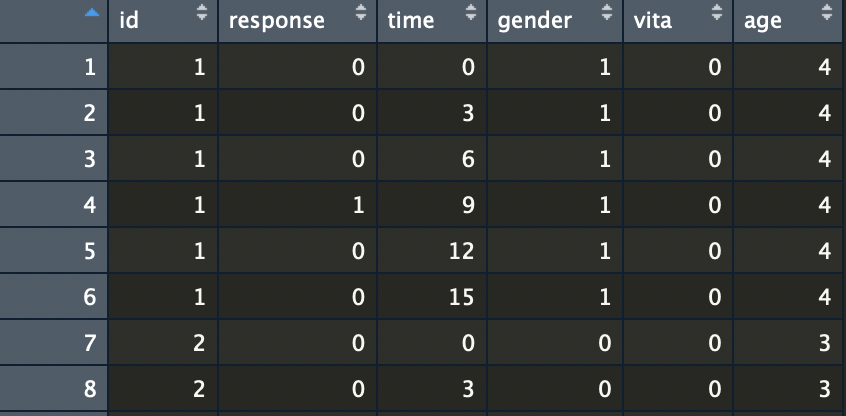
\includegraphics[scale=0.4]{data.png}
	\end{center}
	
	\framebreak
	
	\textbf{Model}\\
	\vspace{2mm}
	$\text{logit Pr}(Y_{ij}=1 \vert U_i) = \text{Pr}(Y_{ij}=1 \vert U_i) / \text{Pr}(Y_{ij}=0 \vert U_i)$ \\
	\vspace{2mm}
	1)  Random intercept				
	\begin{align*}
		 \text{logit Pr}(Y_{ij}=1 \vert U_i) =  \beta_0 + & \beta_1 gender_{ij}+ \beta_2 age_{ij}+ \beta_3 vita_{ij}+	 \beta_4 t_{ij} + U_i,  \\
		 & U_i \sim N(0, \sigma_u^2)		
	\end{align*}
	2)  Random slope 
	\begin{align*}
		 \text{logit Pr}(Y_{ij}=1 \vert U_i) =   \beta_0 & + \beta_1 gender_{ij}+ \beta_2 age_{ij}+ \beta_3 vita_{ij}+	 \beta_4 time_{ij} + U_{i0} + U_{i1}t_{ij}, \\ 
		& \begin{pmatrix}
			U_{i0} \\ U_{i1}
			\end{pmatrix}
			\sim BVN\left(0,
			 \begin{pmatrix}
				\sigma_1^2 & \sigma_{12} \\
				\sigma_{12} & \sigma_2^2
			\end{pmatrix}\right)	
	\end{align*}

	\framebreak
	\textbf{Interpretation} \\
	\begin{itemize}
		\item 랜덤효과 모수 추정치 
			\begin{itemize}
				\item 분산: \underline{클수록 해당 변수의 변이가 큰 것}을 의미\\
				\item 공분산: 양수이면 두 변수가 양의 상관관계, 음수이면 음의 상관관계\\		
			\end{itemize}
		\item 고정효과 모수 추정치
			\begin{itemize}
				\item $i$번째 사람이 비타민 결핍이 아닐 때
					\begin{align*}
						& \exp (\beta_0+U_i) =  \frac{\text{Pr}(Y_{ij}=1 \vert x_{ij}=0, U_i)}{\text{Pr}(Y_{ij}=0 \vert x_{ij}=0, U_i)} 
					\end{align*} 
				\item $i$번째 사람이 비타민 결핍일 때 
				\begin{align*}
					& \exp (\beta_0+ \beta_1 + U_i) =  \frac{\text{Pr}(Y_{ij}=1 \vert x_{ij}=1, U_i)}{\text{Pr}(Y_{ij}=0 \vert x_{ij}=1, U_i)} 
				\end{align*} 
				\item 비타민 결핍 여부에 따른 호흡기 질환에 대한 오즈비 
				\begin{align*}
					\exp (\beta_1) = \frac{\exp(\beta_0 + \beta_1+U_i)}{\exp(\beta_0+U_i)}
				\end{align*}		
			\end{itemize}
	\end{itemize}
	
	\end{frame}
}


\section{Code}{
	\begin{frame}[allowframebreaks]{Code}
		\textbf{R} \\ 
		\vspace{4mm}
		\begin{center}
			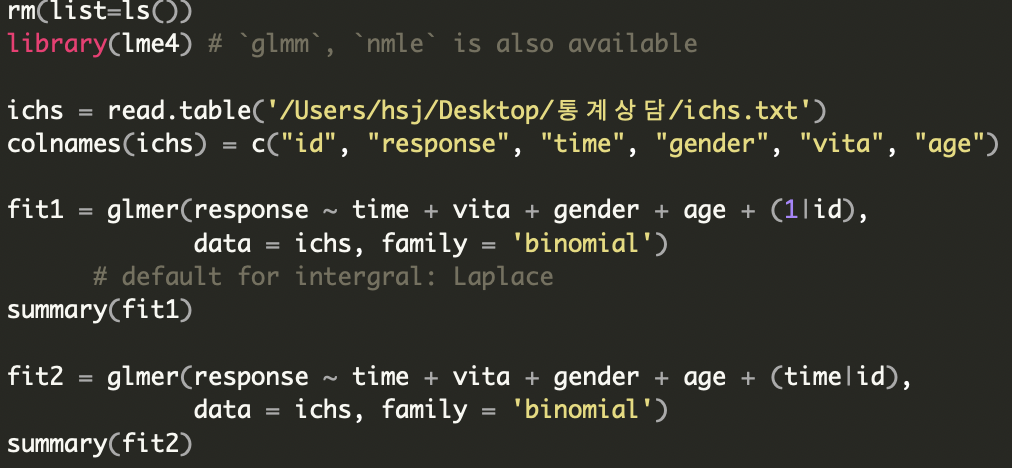
\includegraphics[scale=0.5]{rcode.png} 
		\end{center}
		
		\framebreak
		
		\begin{center}
			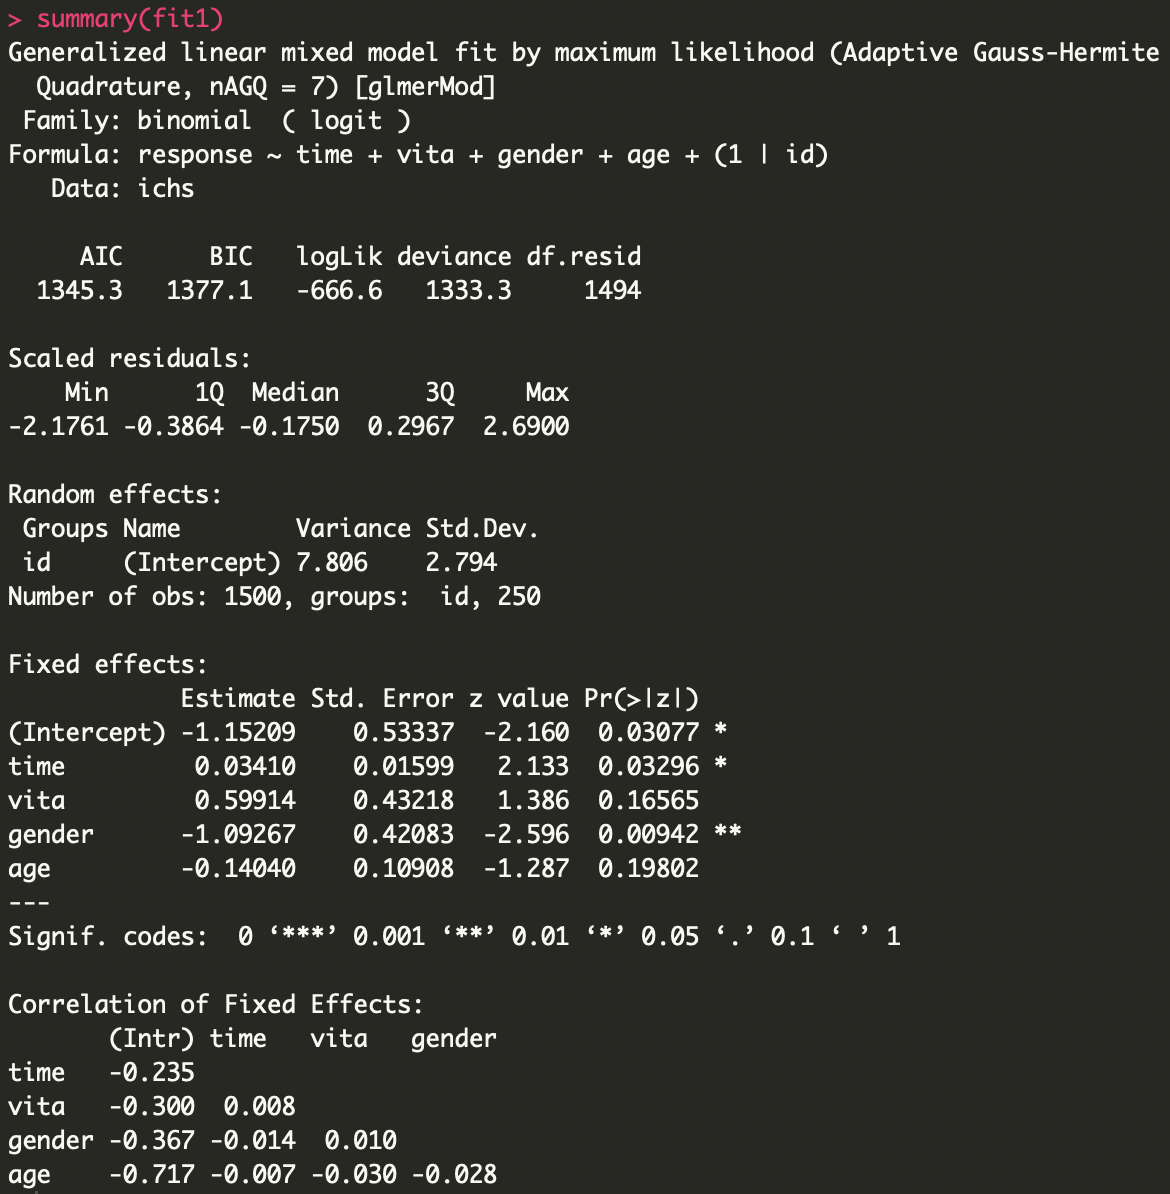
\includegraphics[scale=0.35]{rfit1.png} 
		\end{center} 
	 
		\framebreak
		
		\begin{center}
			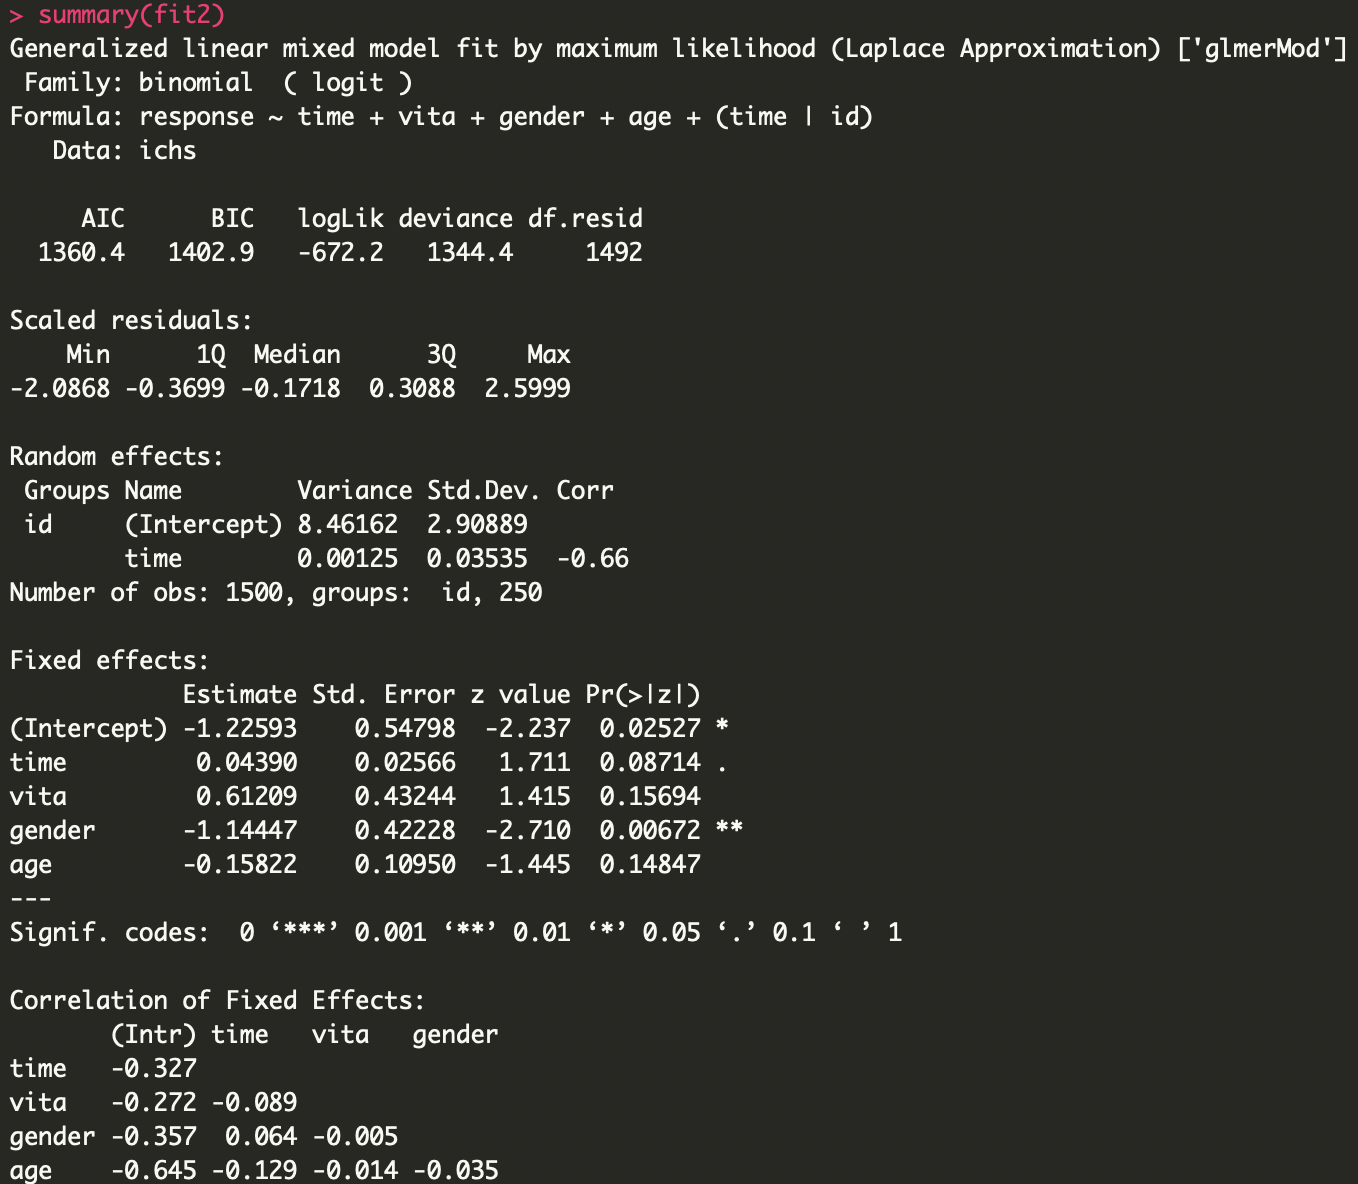
\includegraphics[scale=0.33]{rfit2.png} 
		\end{center}
	
		 \framebreak
			
		\textbf{SAS}
		\vspace{4mm}
		
		\begin{center}
			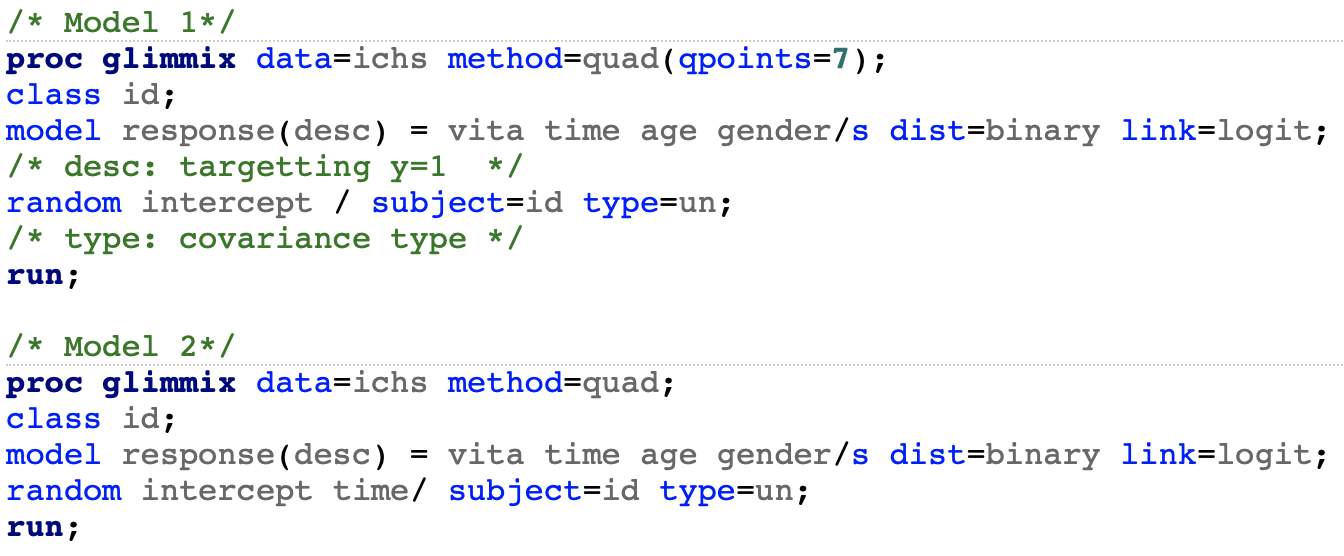
\includegraphics[scale=0.4]{sascode.png} 
		\end{center}
	
		\framebreak
		
		\begin{center}
			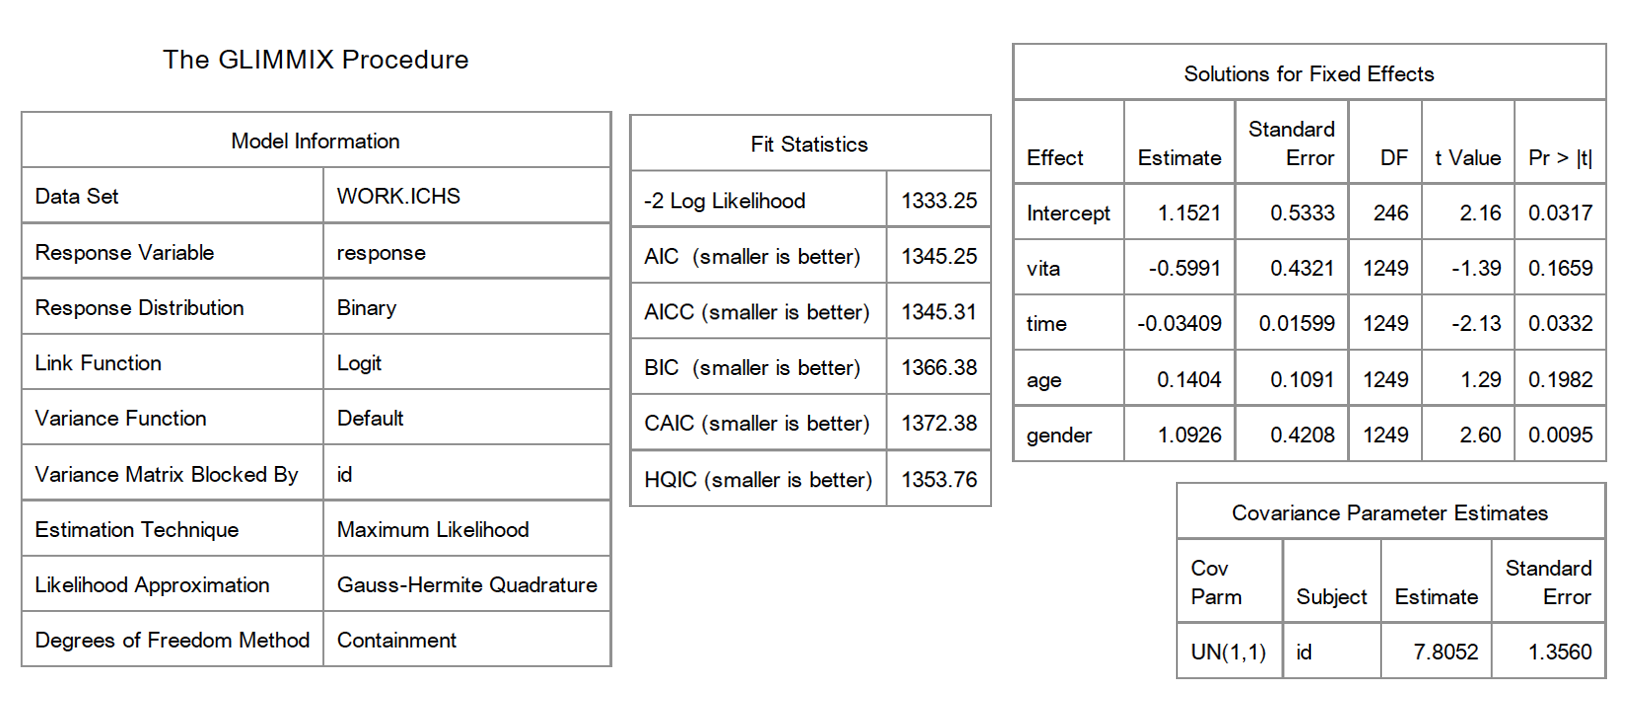
\includegraphics[scale=0.4]{sasfit1.png} 
		\end{center}
	
		\framebreak
	
		\begin{center}
			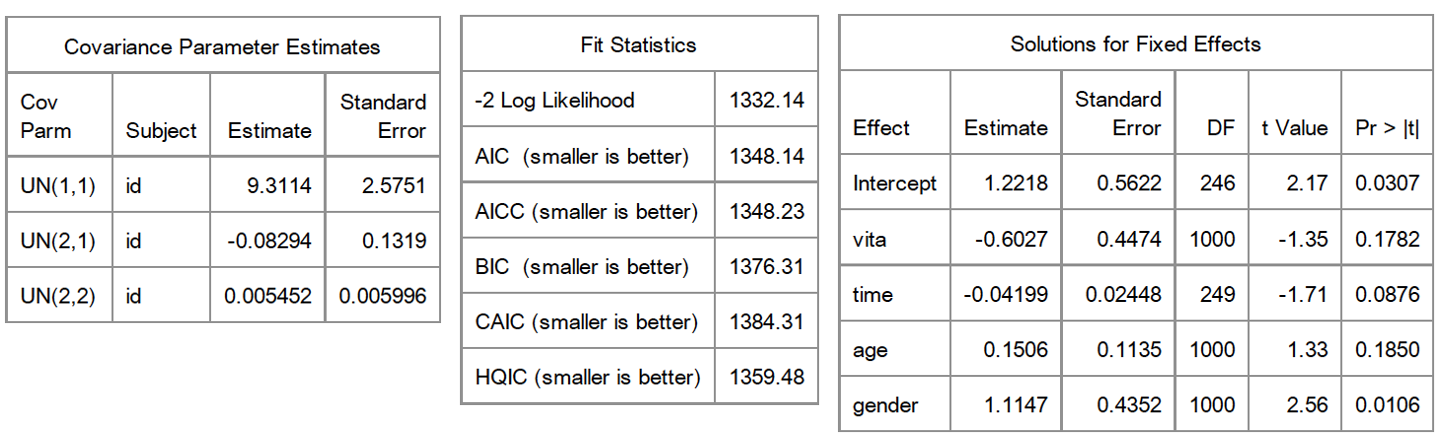
\includegraphics[scale=0.4]{sasfit2.png} 
		\end{center}

		
	\end{frame}
} 
	
%\section{Reference}{
\begin{frame}[allowframebreaks]{Reference}
	\nocite{*} % show references without \cite{}
	\bibliography{ref}
\end{frame}
%}


\end{document}
